%%%%%%%%%%%%%%%%%%%%%%%%%%%%%%%%%%%%%%%%%%%%%%%%%%%%%%%%%%%%%%%%
% Beamer Presentation
% Copyright @ Lu Niu
% School of Physics, University of Sydney
%%%%%%%%%%%%%%%%%%%%%%%%%%%%%%%%%%%%%%%%%%%%%%%%%%%%%%%%%%%%%%%%

%	PACKAGES AND THEMES

\documentclass{beamer}

\mode<presentation> {

% The Beamer class comes with a number of default slide themes, which change the colors and layouts of slides. 
% Below this is a list of all the themes, uncomment each in turn to see what they look like.

%\usetheme{default}
%\usetheme{AnnArbor}
%\usetheme{Antibes}
%\usetheme{Bergen}
%\usetheme{Berkeley}
%\usetheme{Berlin}
%\usetheme{Boadilla}
%\usetheme{CambridgeUS}
%\usetheme{Copenhagen}
%\usetheme{Darmstadt}
%\usetheme{Dresden}
%\usetheme{Frankfurt}
%\usetheme{Goettingen}
%\usetheme{Hannover}
%\usetheme{Ilmenau}
%\usetheme{JuanLesPins}
%\usetheme{Luebeck}
\usetheme{Madrid}
%\usetheme{Malmoe}
%\usetheme{Marburg}
%\usetheme{Montpellier}
%\usetheme{PaloAlto}
%\usetheme{Pittsburgh}
%\usetheme{Rochester}
%\usetheme{Singapore}
%\usetheme{Szeged}
%\usetheme{Warsaw}

% As well as themes, the Beamer class has a number of color themes for any slide theme. 
% Uncomment each of these in turn to see how it changes the colors of your current slide theme.

%\usecolortheme{albatross}
%\usecolortheme{beaver}
%\usecolortheme{beetle}
%\usecolortheme{crane}
%\usecolortheme{dolphin}
%\usecolortheme{dove}
%\usecolortheme{fly}
%\usecolortheme{lily}
%\usecolortheme{orchid}
%\usecolortheme{rose}
%\usecolortheme{seagull}
%\usecolortheme{seahorse}
%\usecolortheme{whale}
%\usecolortheme{wolverine}

%\setbeamertemplate{footline} % To remove the footer line in all slides uncomment this line
%\setbeamertemplate{footline}[page number] % To replace the footer line in all slides with a simple slide count uncomment this line

%\setbeamertemplate{navigation symbols}{} % To remove the navigation symbols from the bottom of all slides uncomment this line
}

\usepackage{graphicx} % Allows including images
\usepackage{booktabs} % Allows the use of \toprule, \midrule and \bottomrule in tables
\usepackage{braket}

%	TITLE PAGE

\title[Short title]{Effect of external field on the I-V characteristics through the molecular nano-junction} % The short title appears at the bottom of every slide, the full title is only on the title page

\author{Lu Niu} % Your name
\institute[USYD] % Your institution as it will appear on the bottom of every slide, may be shorthand to save space
{
The University of Sydney \\ % Your institution for the title page
\medskip
\textit{luke.niu@sydney.edu.au} % Your email address
}
\date{\today} % Date, can be changed to a custom date

\begin{document}

\begin{frame}
\titlepage % Print the title page as the first slide
\end{frame}

\begin{frame}
\frametitle{Overview} % Table of contents slide, comment this block out to remove it
\tableofcontents % Throughout your presentation, if you choose to use \section{} and \subsection{} commands, these will automatically be printed on this slide as an overview of your presentation
\end{frame}

%	PRESENTATION SLIDES


\section{Introduction} % Sections can be created in order to organize your presentation into discrete blocks, all sections and subsections are automatically printed in the table of contents as an overview of the talk

    \subsection{Background}

\begin{frame}
\frametitle{Background}
As the basic functional unit of molecular electronics, the structure of single molecular nano-junction sandwiched between Nano-electrodes has been attracted many interests in molecular science. The charge transmission dynamics problems received increasing attention and have been subsequently studied extensively, in particular, its current voltage (IV) characteristics induced by an external field.
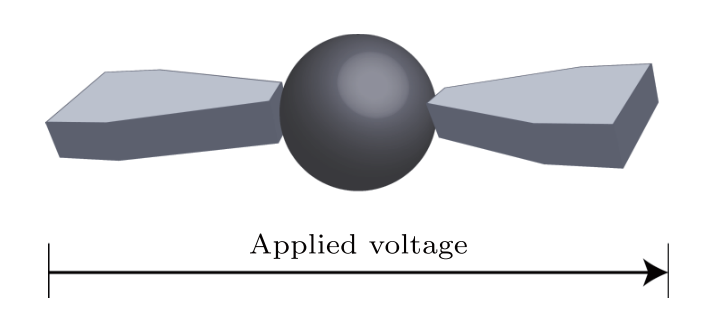
\includegraphics[scale=0.4]{NanoJunction.png}
\end{frame}

    \subsection{Theoretical Method}

\begin{frame}
\frametitle{Method Section}
In the system of molecular nano-junction which composed by a molecule between a pair of leads, with the method of extended General Master Equation, the characteristic curves of stationary and transient current have been computed and explained theoretically. It is found that the current can be evidently controlled via some factors adjustments, such as external field, the relaxation of molecules, intra-molecular vibration energy redistribution, and others.
\end{frame}

\begin{frame}
\frametitle{Theoretical Model Description}
    The introduced electron-vibrational states, are used for an expansion of the overall molecular junction Hamiltonian:
\begin{equation}
    H = H_{mol} + H_{lead} + H_{mol-lead} + H_{mol-field}
\end{equation}
    The Hamiltonian of the molecular part:
\begin{equation}
    H_{mol} = \sum_{\alpha}\hbar\varepsilon_{\alpha}\ket{\psi_\alpha}\bra{\psi_\alpha}+\sum_{\alpha\beta}W_{\alpha\beta}\ket{\psi_\alpha}\bra{\psi_\beta}
\end{equation}
The quadratic quantized form of the Hamiltonian of leads:
\begin{equation}
    H_{lead} = \sum_{X=L,R}H_{lead}^X = \sum_{X=L,R}\sum_{k,s}\hbar\omega_{Xks}\alpha^\dagger_{Xks}\alpha_{Xks}
\end{equation}

\end{frame}

\begin{frame}
\frametitle{Theoretical Model Description: Hamiltonian}
The Hamiltonian of the interaction between the leads and the molecule:
\begin{equation}
\begin{split}
    H_{mol-lead}= & \sum_{X=L,R}\sum_{k,s}T_X(N+1a,Nb,ks)\times\alpha_{Xks}\ket{\varphi_{N+1a}}\bra{\varphi_{Nb}}  \\
    + & \sum_{X=L,R}\sum_{k,s}T_X(Na,N+1b,ks)\times\alpha_{Xks}\ket{\varphi_{Na}}\bra{\varphi_{N+1b}} 
\end{split}
\end{equation}
\end{frame}

\begin{frame}
\frametitle{Theoretical Model Description}
The coupling to the external optical field:
\begin{equation}
    H_{mol-field}(t)=-\sum_{\alpha,\beta}\ket{\alpha}\bra{\beta}\vec{d}_{\alpha\beta}\cdot\vec{E}(t)
\end{equation}
The filed form:
\begin{equation}
    \vec{E}(t) = \vec{n}\cdot E(t)e^{-i\omega t} + c.c.
\end{equation}
The general form of rate equation:
\begin{equation}
    \frac{\partial}{\partial t} P_{\alpha}(t) = -\sum_{\beta}\left[P_{\alpha}(t) K_{\alpha\rightarrow\beta}(t)-P_{\beta}(t) K_{\beta\rightarrow \alpha}(t)\right]
\end{equation}
\end{frame}

\section{Result}

    \subsection{Numerical Simulation}

\begin{frame}
\frametitle{Numerical Simulation}
Due to the strong electronic-vibrational coupling, the IV curves have the inelastic character in the molecular nanojunction and the stationary current increase as steps with the applied bias voltage. The Franck-Condon blockage can be effectively removed by the application of coupled external field. Applying Gaussian pulse widths of different orders of magnitude, the stationary current in the molecule needs different time period has been revealed on our work. Thought system described and computed, we got results of current curves with varying voltages applied as shown in Fig.1, and different magnitudes of pulse width as shown in Fig.2.  
\end{frame}

\begin{frame}
\frametitle{Numerical Simulation}
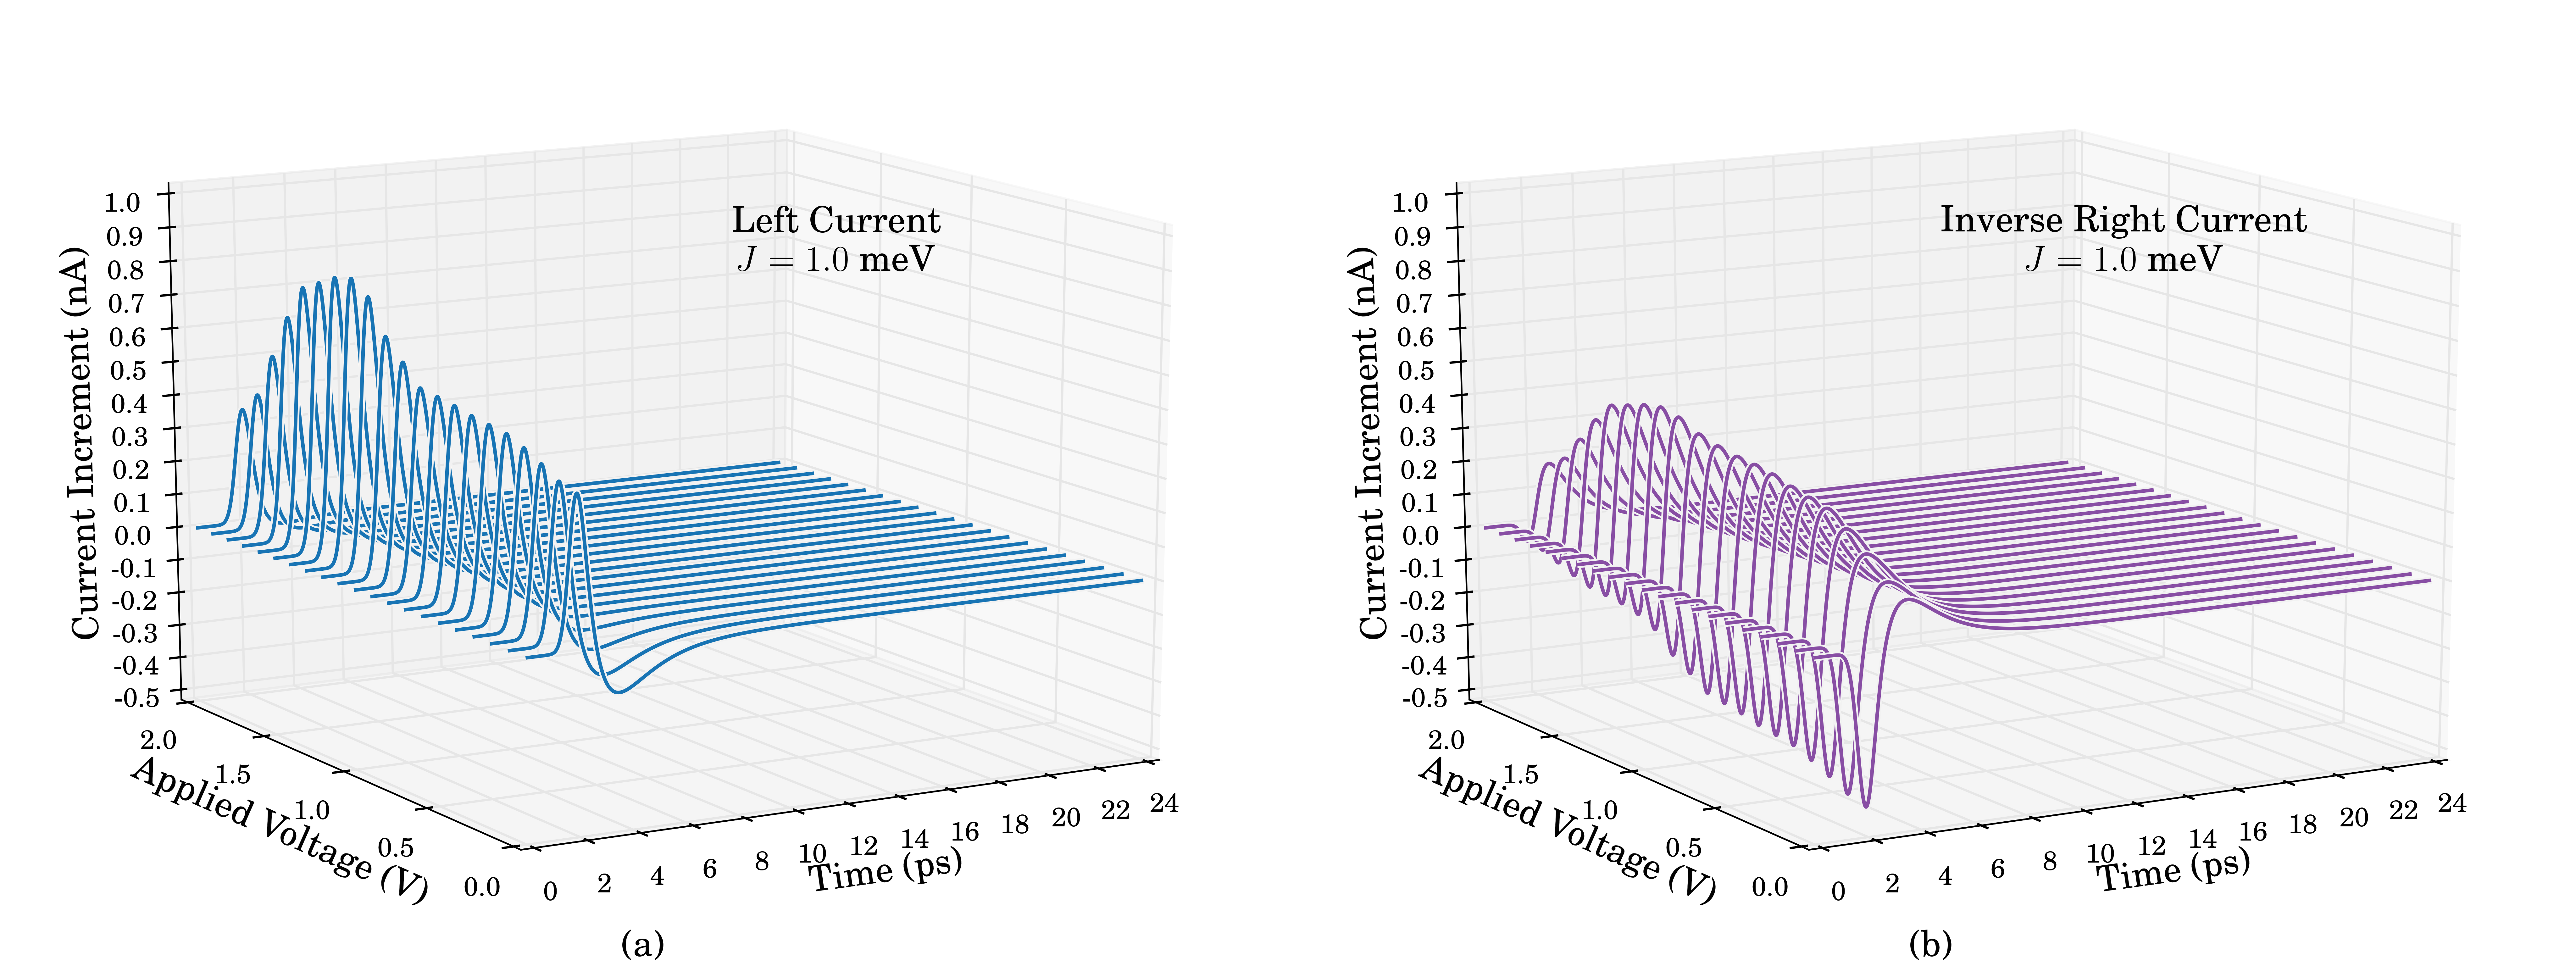
\includegraphics[scale=0.05]{F1.png}
\par Fig.1: Applied a Gaussian external field and the bias voltage between 0-2V with the coefficient of IVR at 1.0meV, the transient IV characteristic curves are demonstrated: (a) the transient current from left lead to molecule; (b) the transient current from the right lead to molecule. 
\end{frame}

\begin{frame}
\frametitle{Numerical Simulation}
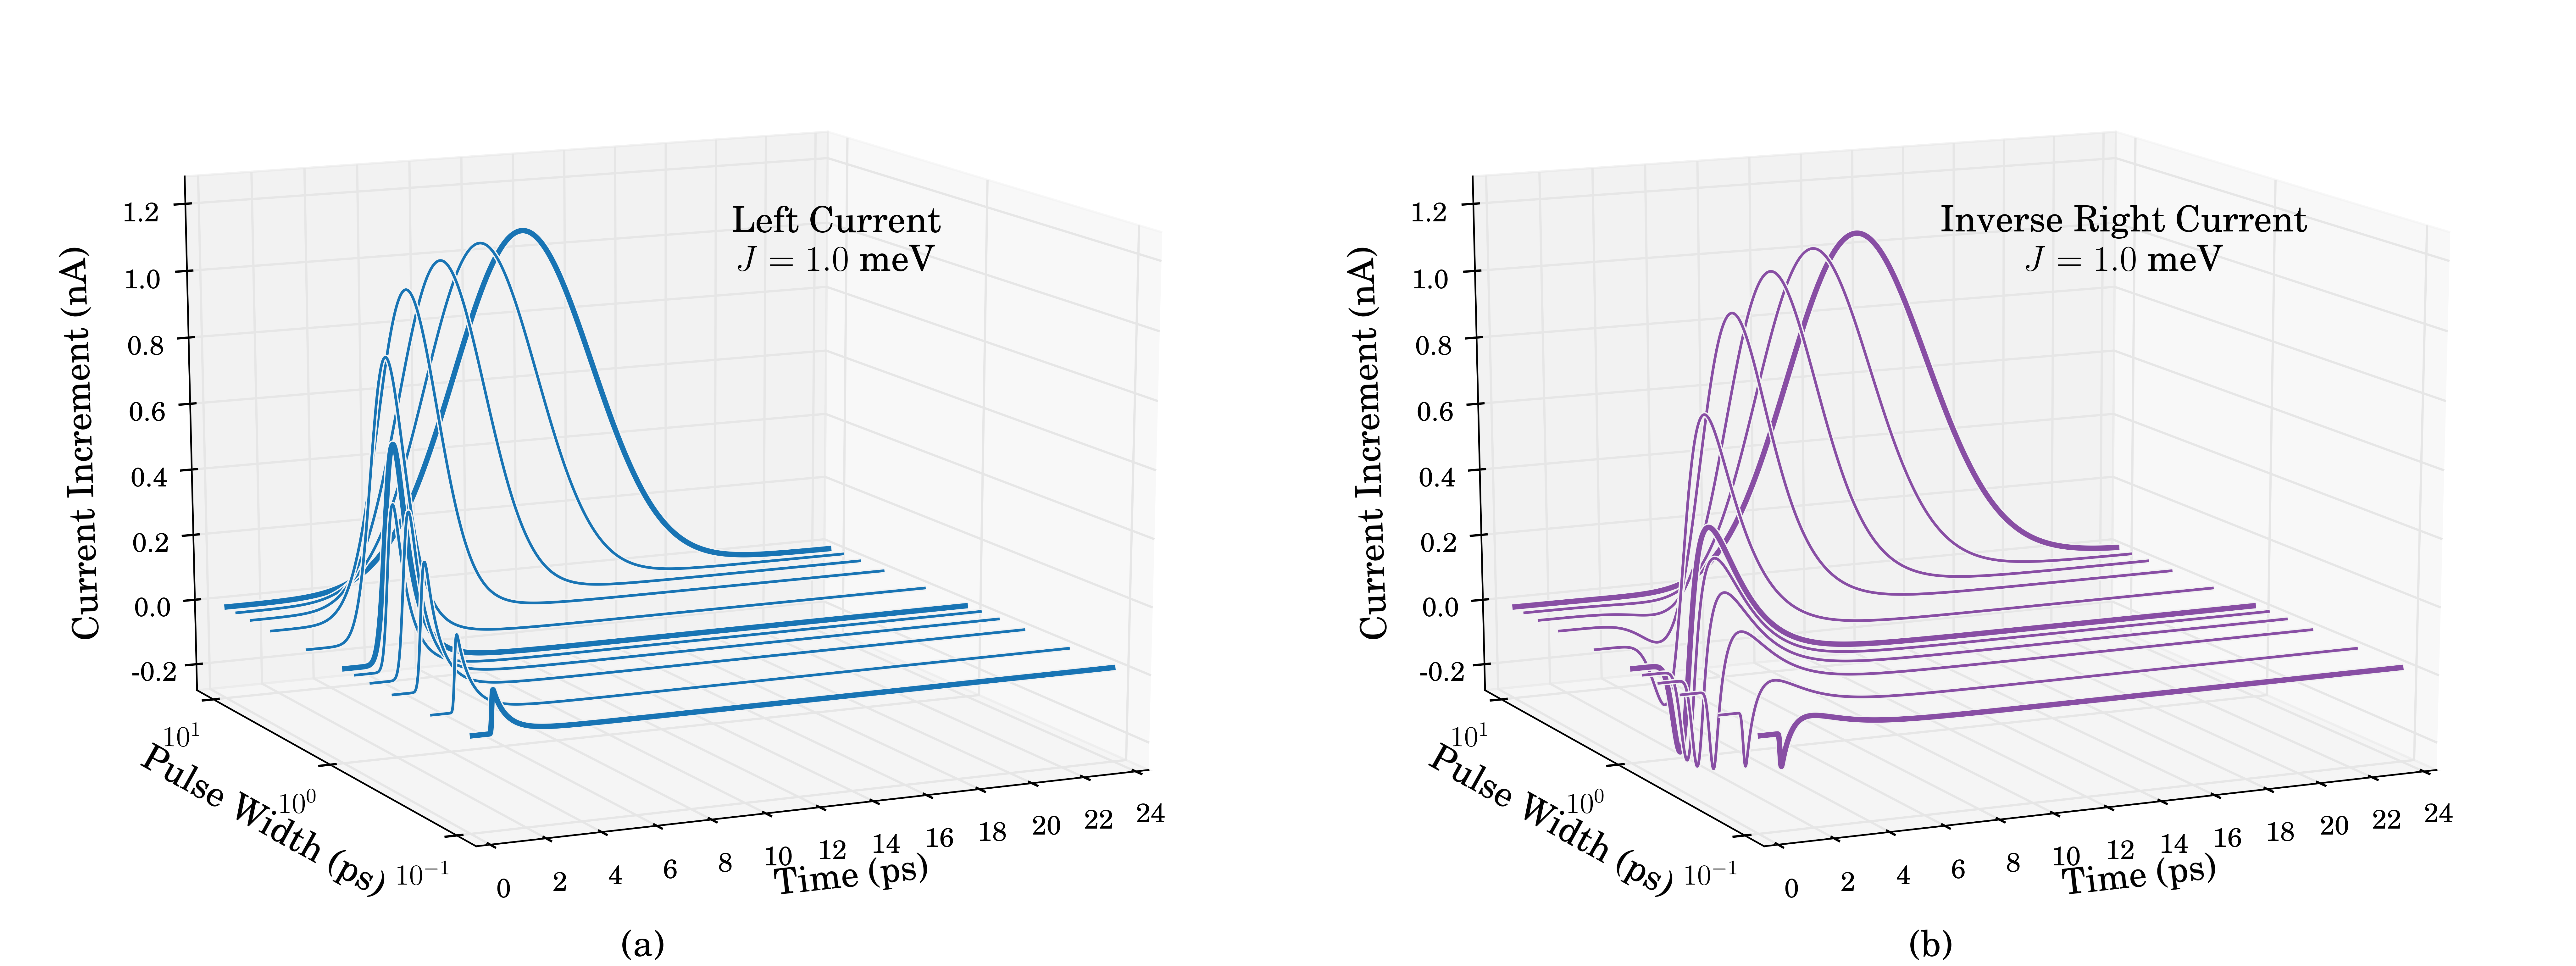
\includegraphics[scale=0.05]{F2.png}
\par Fig.2: With the applied bias voltage of 1V and the coefficient of IVR at 1.0meV, the left and right transient current curves are plotted for various pulse widths of Gaussian external field. From the front to back, pulse widths are 0.1ps(bold), 0.2ps, 0.4ps, 0.6ps, 0.8ps, 1.0ps(bold), 2ps, 4ps, 6ps, 8ps, 10ps(bold) respectively. 
\end{frame}

    \subsection{Result Analysis}

\begin{frame}
\frametitle{Result Analysis}
It is obviously that the transient current with its left part different with the right part is very significant for the 1ps width pulse excitation. In this case, the system stays in the state of non-equilibrium. However, with pulse width and applied voltage increasing, the current through the molecular nanojunction tends to be equilibrium.
\end{frame}

\begin{frame}
\Huge{\centerline{Thank You}}
\end{frame}

\end{document} 